\documentclass[11pt,a4paper]{article}

% =====================================================
% PACKAGES
% =====================================================
\usepackage[utf8]{inputenc}
\usepackage[T1]{fontenc}
\usepackage[french]{babel}
\usepackage{lmodern}
\usepackage{geometry}
\usepackage{xcolor}
\usepackage{graphicx}
\usepackage{booktabs}
\usepackage{tabularx}
\usepackage{array}
\usepackage{float}
\usepackage{hyperref}
\usepackage{listings}
\usepackage{fancyhdr}
\usepackage{titlesec}
\usepackage{enumitem}

\geometry{
    top=2.1cm,
    bottom=2.1cm,
    left=2.3cm,
    right=2.3cm
}

\definecolor{mainblue}{HTML}{163A59}
\definecolor{lightgray}{HTML}{F3F5F7}
\definecolor{codegreen}{HTML}{287C46}

\hypersetup{
    colorlinks=true,
    linkcolor=mainblue,
    urlcolor=mainblue
}

\titleformat{\section}
{\Large\bfseries\color{mainblue}}
{\thesection}{0.7em}{}

\titleformat{\subsection}
{\large\bfseries}
{\thesubsection}{0.7em}{}

\lstdefinestyle{terminal}{
    basicstyle=\ttfamily\footnotesize,
    backgroundcolor=\color{lightgray},
    frame=single,
    rulecolor=\color{gray!35},
    breaklines=true,
    columns=fullflexible,
    keepspaces=true,
    showstringspaces=false,
    keywordstyle=\color{codegreen},
    xleftmargin=5pt,
    xrightmargin=5pt
}

\lstset{style=terminal}

\pagestyle{fancy}
\fancyhf{}
\lhead{\small VM Siemens TIA Portal}
\rhead{\small VMware -- Windows 10 -- Siemens}
\cfoot{\thepage}
\setlength{\headheight}{14pt}

% =====================================================
% DOCUMENT
% =====================================================

\begin{document}

\begin{titlepage}
    \centering
    \vspace*{3cm}

    {\Huge\bfseries
    Installation et configuration\\[0.3cm]
    de la VM Siemens TIA Portal
    \par}

    \vspace{1cm}

    {\Large
    Poste logiciel d'automatisme pour le laboratoire OT--IT
    \par}

    \vspace{1.5cm}

    {\large
    VMware Workstation -- Windows 10 -- TIA Portal -- STEP 7 -- WinCC
    \par}

    \vfill

    \begin{tabular}{rl}
        Machine virtuelle : & \texttt{Siemens\_TIA\_STEP7\_Win10} \\
        Systeme invite : & Windows 10 Pro 22H2, build 19045.6093 \\
        Plateforme hote : & Lenovo LOQ / VMware Workstation \\
        Date des captures : & Octobre 2026 \\
    \end{tabular}

    \vspace{2cm}

    {\large Documentation technique prete pour Overleaf et GitHub}

\end{titlepage}

\tableofcontents
\newpage

% =====================================================
\section{Objectif du document}
% =====================================================

Ce document decrit l'installation de la machine virtuelle utilisee
comme poste Siemens dans le laboratoire. Il couvre la preparation de
Windows, l'installation des logiciels Siemens observes dans les captures,
les reglages realises, les incidents rencontres et les validations
disponibles.

Le document est volontairement separe de la documentation
Windows Server / Active Directory. La VM Siemens sera ensuite reliee au
reseau OT prive et au domaine \texttt{ad.lab}, mais ce raccordement est
documente dans le deuxieme livrable.

Les projets Ignition et AVEVA sont des etapes futures. Ils ne sont pas
presentes ici comme installes.

% =====================================================
\section{Etat verifie et points a confirmer}
% =====================================================

\begin{table}[H]
\centering
\begin{tabularx}{\textwidth}{lX}
\toprule
\textbf{Etat} & \textbf{Element} \\
\midrule
Verifie & La VM \texttt{Siemens\_TIA\_STEP7\_Win10} demarre dans VMware Workstation. \\
Verifie & Windows 10 Pro version 22H2, build 19045.6093, est visible dans la VM. \\
Verifie & TIA Portal STEP 7 Professional / WinCC Professional V15.1 Update 5 a ete telecharge et lance. \\
Verifie & Le portail TIA V15.1 s'ouvre et permet la creation d'un projet. \\
Verifie & Plusieurs composants Siemens sont presents dans les programmes installes. \\
Verifie & STEP 7 V5.7 incl. SP2 a ete lance en installation standard. \\
A confirmer & Les ressources exactes de la VM, comme RAM, vCPU et taille disque, ne sont pas visibles dans les captures exploitees. \\
A confirmer & L'etat de licence final de STEP 7 V5.7 doit etre controle dans Automation License Manager. \\
\bottomrule
\end{tabularx}
\caption{Synthese entre elements confirmes et elements a confirmer}
\end{table}

% =====================================================
\section{Creation de la VM et installation Windows}
% =====================================================

\subsection{Role de la VM}

La VM Siemens sert de poste d'ingenierie pour les logiciels
d'automatisme. Elle permet de travailler dans un environnement separe
du PC hote, tout en conservant la possibilite de communiquer avec les
autres machines du laboratoire via VMware.

Dans l'etat actuel, les captures ne permettent pas de confirmer les
valeurs exactes de processeur, memoire et disque. Pour publication
GitHub, ces valeurs devront etre completees apres verification dans les
parametres VMware de la VM.

\subsection{Systeme Windows installe}

La capture suivante confirme l'environnement Windows observe dans la VM :
Windows 10 Professionnel, version 22H2, build 19045.6093.

\begin{figure}[H]
    \centering
    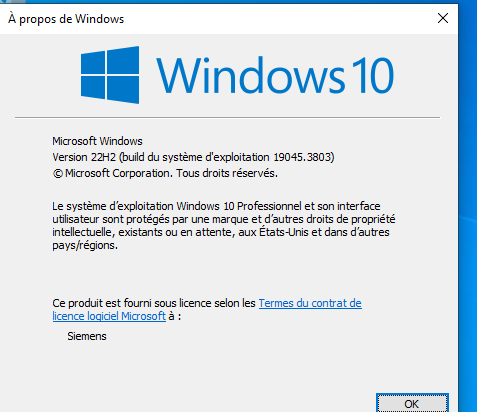
\includegraphics[width=0.82\textwidth]{images/tia-01-windows-10-version.png}
    \caption{Version Windows 10 Pro observee dans la VM Siemens.}
\end{figure}

\subsection{Bonnes pratiques retenues}

\begin{itemize}[leftmargin=*]
    \item garder la VM Siemens separee du serveur Active Directory ;
    \item utiliser VMware Tools pour l'integration de la VM avec l'hote ;
    \item conserver des captures et notes d'installation pour chaque logiciel Siemens ;
    \item eviter d'inclure des licences, identifiants ou mots de passe dans le depot GitHub ;
    \item completer les ressources materielles exactes avant publication finale.
\end{itemize}

% =====================================================
\section{Installation TIA Portal V15.1 Update 5}
% =====================================================

\subsection{Telechargement Siemens}

Les captures montrent le telechargement de
TIA Portal STEP 7 Professional / WinCC Professional V15.1 Update 5.
Le paquet etait decoupe en plusieurs parties, avec une verification
SHA-256 disponible cote Siemens.

\begin{figure}[H]
    \centering
    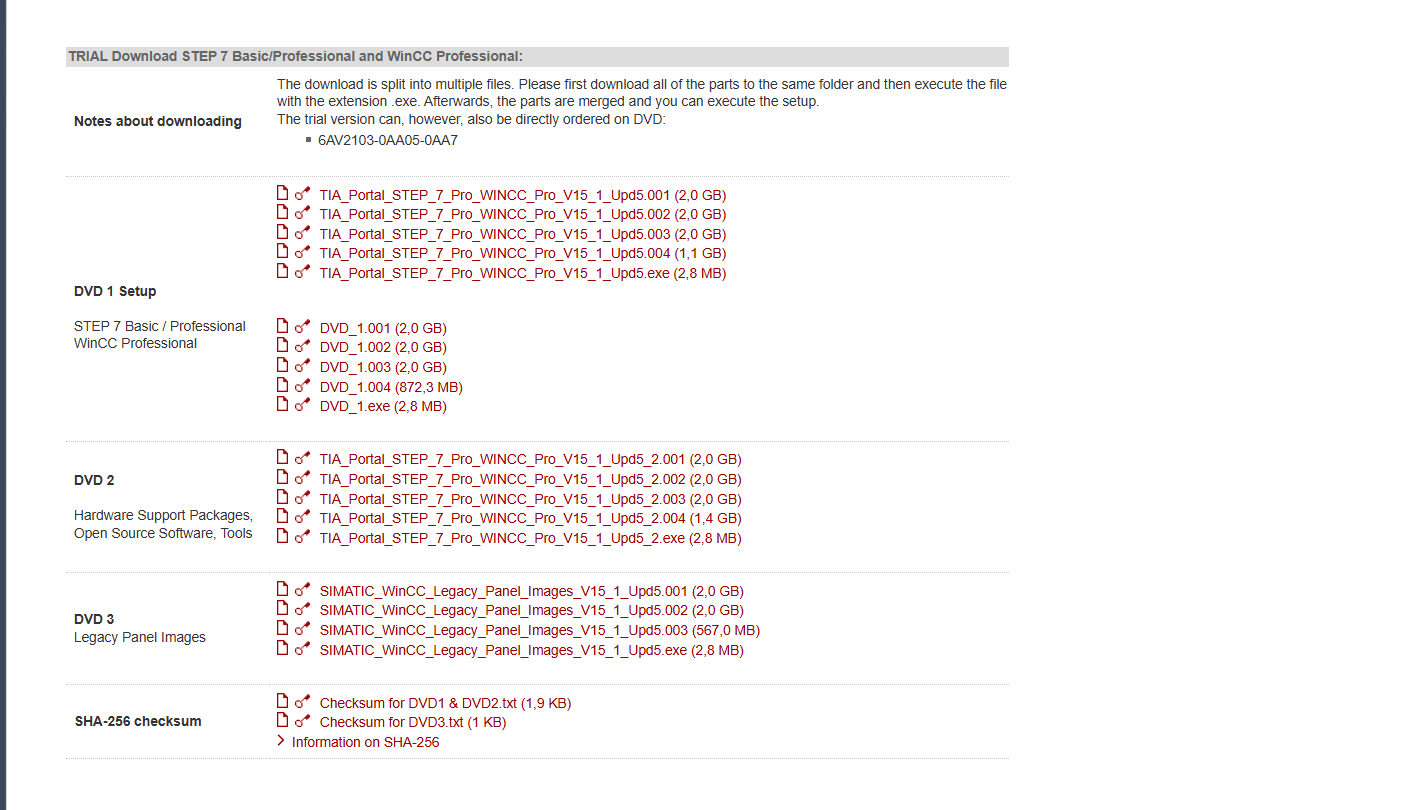
\includegraphics[width=\textwidth]{images/tia-02-telechargement-tia-v151-upd5.png}
    \caption{Page de telechargement TIA Portal STEP 7 Professional / WinCC Professional V15.1 Update 5.}
\end{figure}

\subsection{Configuration du produit}

L'assistant d'installation TIA Portal a ete lance avec la configuration
typique. La selection visible contient notamment :
\texttt{SIMATIC STEP 7 Professional V15.1 Upd5},
\texttt{SIMATIC WinCC Professional V15.1 Upd5}, les composants
WinCC Engineering System, WinCC Runtime Advanced et les composants de
simulation.

\begin{figure}[H]
    \centering
    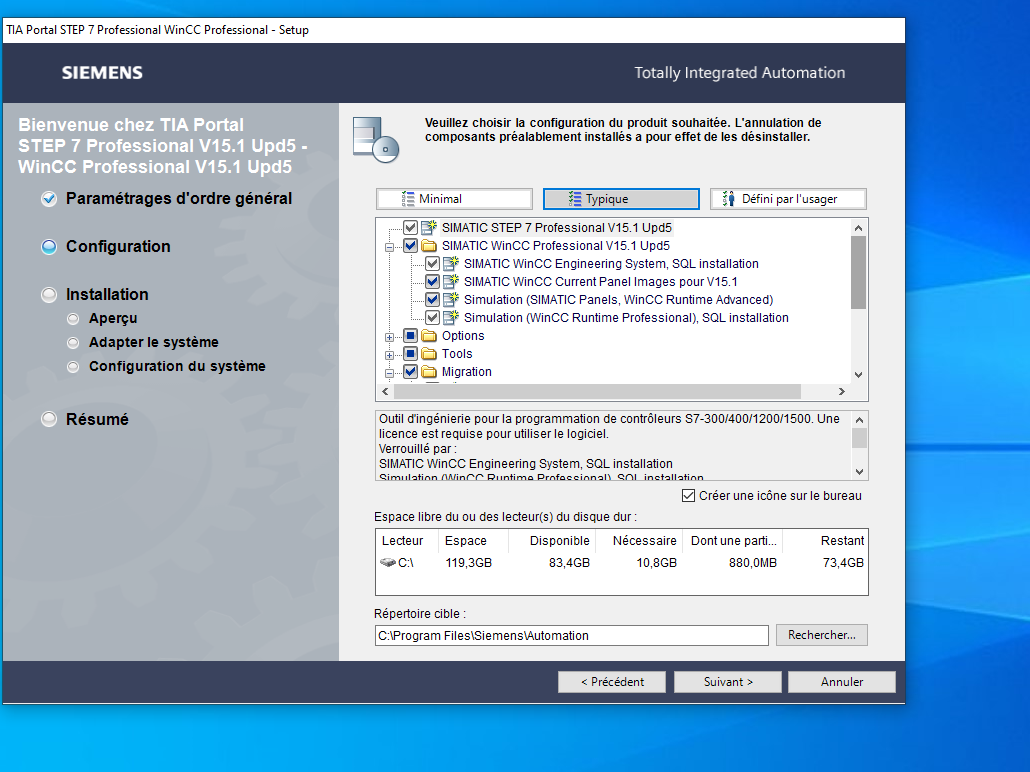
\includegraphics[width=0.88\textwidth]{images/tia-03-configuration-produit-tia.png}
    \caption{Selection des composants TIA Portal et WinCC Professional V15.1 Update 5.}
\end{figure}

\subsection{Incident d'installation}

Un incident est apparu pendant l'installation, dans l'etape
\og Adapter le systeme \fg{}. L'assistant Siemens demandait un
redemarrage de l'ordinateur pour poursuivre ou finaliser l'installation.

\begin{figure}[H]
    \centering
    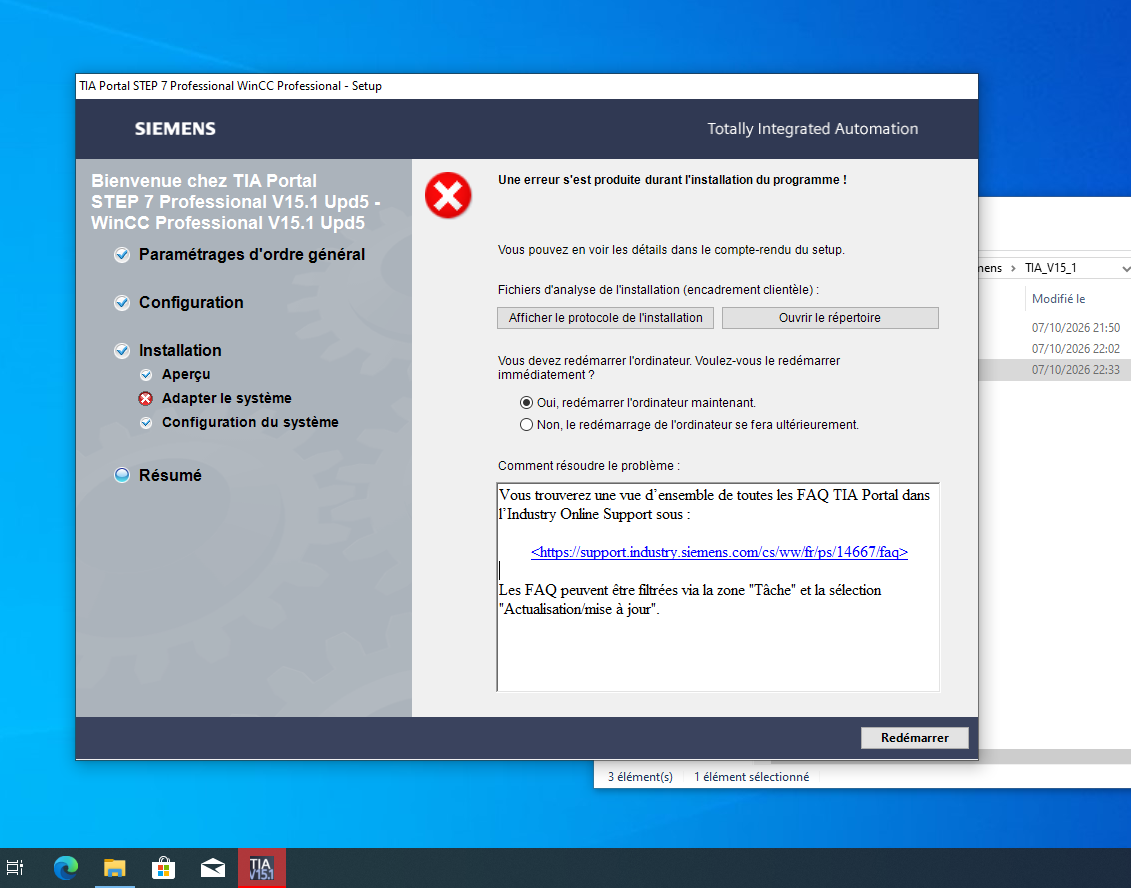
\includegraphics[width=0.86\textwidth]{images/tia-04-incident-redemarrage-installation.png}
    \caption{Incident Siemens demandant un redemarrage pendant l'installation.}
\end{figure}

La resolution retenue est simple : redemarrer la VM, reprendre les
verifications apres redemarrage, puis confirmer dans Windows que les
programmes Siemens attendus sont presents.

% =====================================================
\section{Logiciels Siemens observes apres installation}
% =====================================================

\subsection{Raccourcis visibles sur le bureau}

Apres installation, le bureau Windows montre les raccourcis Siemens
\texttt{Automation License Manager} et \texttt{TIA Administrator}.

\begin{figure}[H]
    \centering
    
\includegraphics[width=0.86\textwidth]{images/tia-05-bureau-outils-siemens.png}
    \caption{Raccourcis Siemens visibles sur le bureau de la VM.}
\end{figure}

\subsection{Programmes Siemens installes}

La liste \og Programmes et fonctionnalites \fg{} confirme plusieurs
composants Siemens. Les versions sont recopiees uniquement quand elles
sont visibles dans la capture.

\begin{table}[H]
\centering
\begin{tabularx}{\textwidth}{lX}
\toprule
\textbf{Logiciel / composant} & \textbf{Version observee} \\
\midrule
Siemens Automation License Manager V6.0 + SP8 & 06.00.0800 \\
SIMATIC ProSave V16.0 Upd1 & 16.00.0001 \\
SIMATIC WinCC Runtime Advanced V15.1 Upd5 & V15.1 Upd5 \\
TIA Administrator & V1.0 \\
TIA Portal Multiuser Server V15.1 & V15.1 Upd5 \\
User Management Component & V1.9 SP1 UPD6 \\
OPC .NET API 2.00 Redistributables & 2.00.10200 / 2.01.10600 \\
OPC Core Components Redistributable & 3.00.10600 / 3.00.10102 \\
Microsoft SQL Server 2014 et composants SQL & presents, versions visibles dans Windows \\
VMware Tools & 13.1.5.0 \\
\bottomrule
\end{tabularx}
\caption{Composants effectivement visibles dans les programmes installes}
\end{table}

\begin{figure}[H]
    \centering
    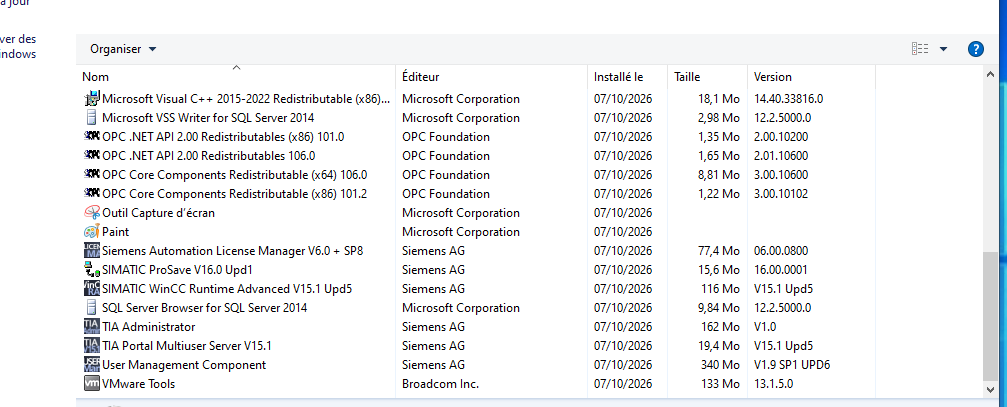
\includegraphics[width=\textwidth]{images/tia-06-programmes-siemens-installes.png}
    \caption{Composants Siemens observes dans les programmes installes.}
\end{figure}

\begin{figure}[H]
    \centering
    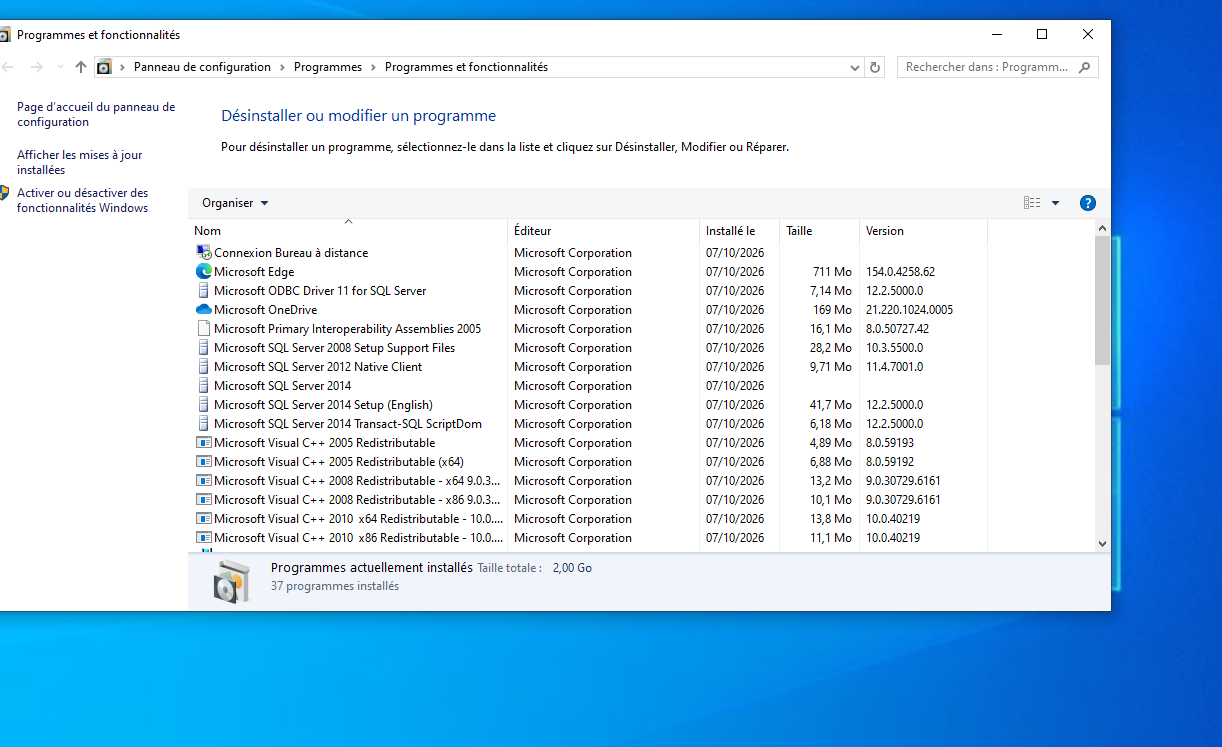
\includegraphics[width=\textwidth]{images/tia-07-programmes-composants-microsoft.png}
    \caption{Composants Microsoft et SQL installes avec l'environnement Siemens.}
\end{figure}

% =====================================================
\section{Validation de TIA Portal}
% =====================================================

\subsection{Ouverture du portail}

La validation principale consiste a ouvrir TIA Portal et a atteindre
l'ecran de creation de projet. La capture montre le portail
Totally Integrated Automation avec la version \texttt{V15.1}.

\begin{figure}[H]
    \centering
    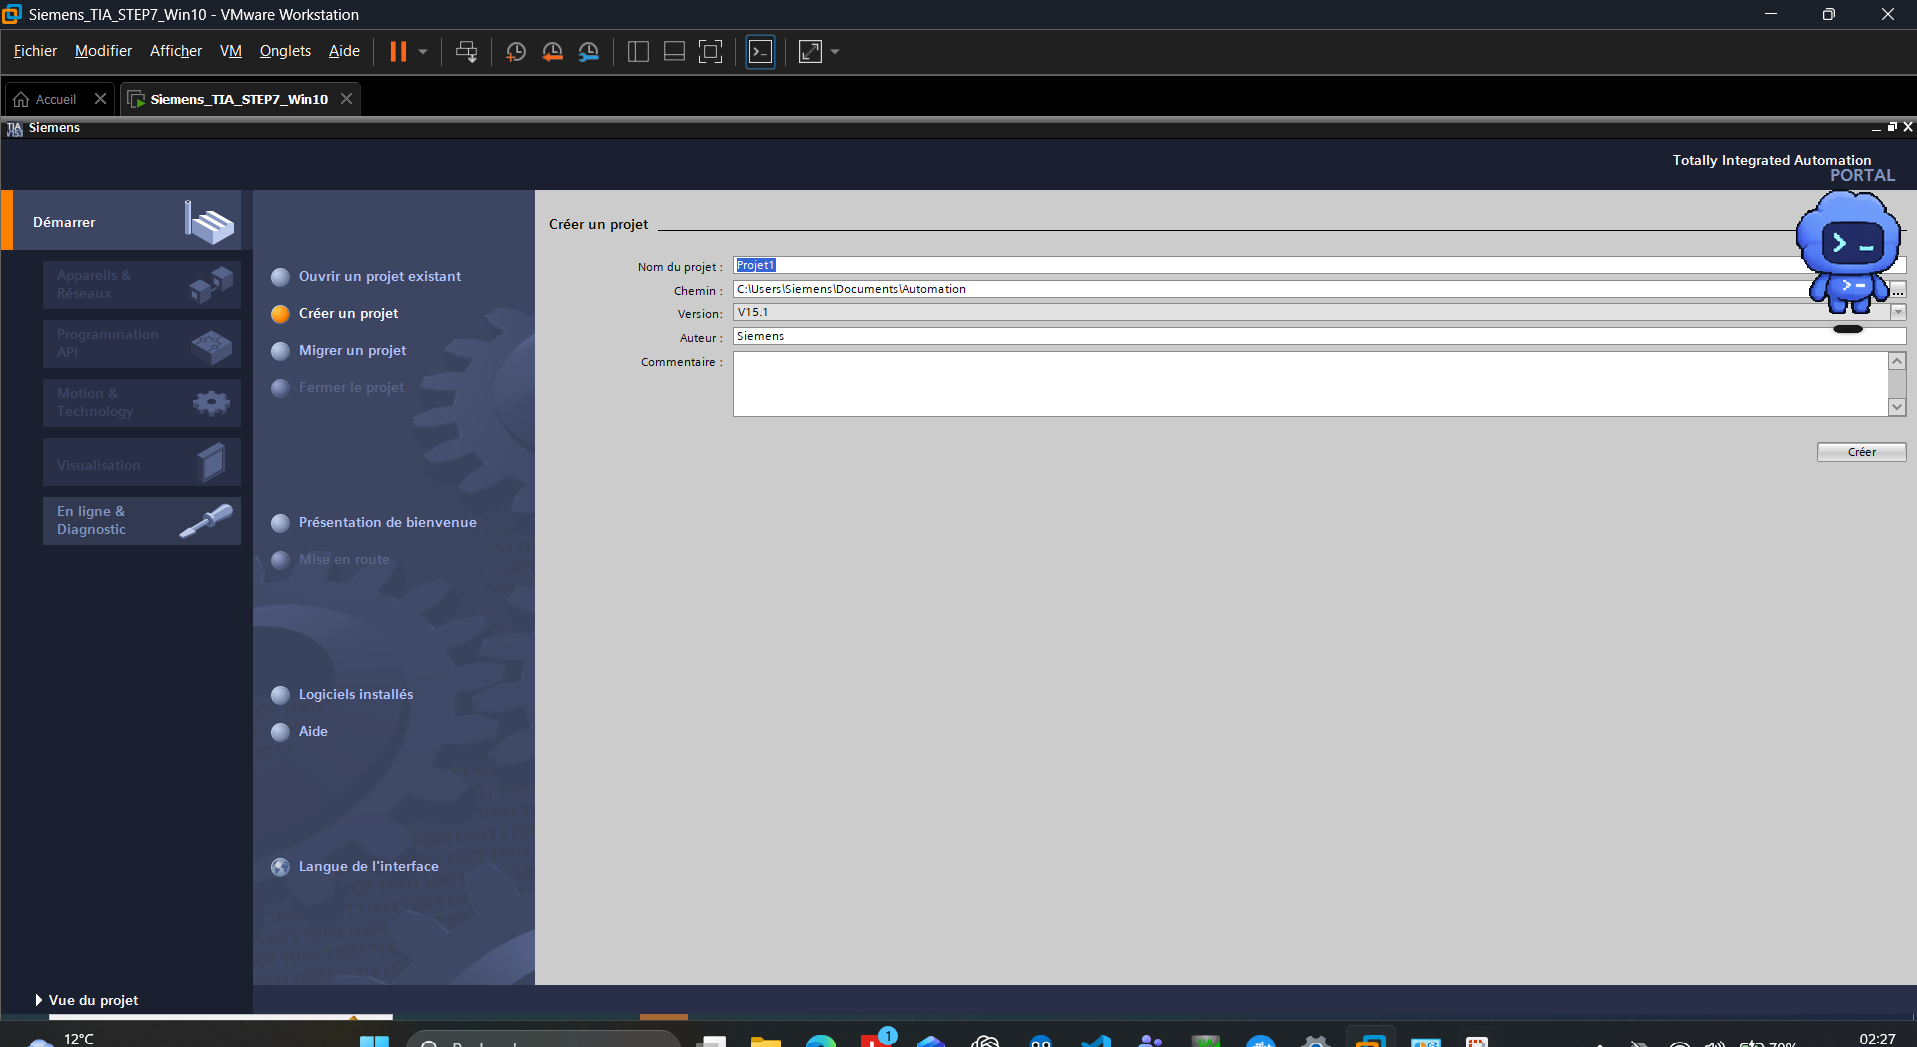
\includegraphics[width=\textwidth]{images/tia-08-portail-tia-creation-projet.png}
    \caption{TIA Portal ouvert dans la VM avec creation de projet disponible.}
\end{figure}

\subsection{Test minimal recommande}

Pour completer la validation avant publication GitHub, il est recommande
de faire un test minimal non connecte a un automate reel :

\begin{lstlisting}
1. Ouvrir TIA Portal.
2. Creer un projet de test local.
3. Verifier que le projet est cree dans Documents\Automation.
4. Fermer puis rouvrir le projet.
5. Noter la version exacte affichee dans Aide > A propos.
\end{lstlisting}

Ce test ne necessite aucun mot de passe ni licence publiee dans le depot.

% =====================================================
\section{Installation STEP 7 V5.7}
% =====================================================

\subsection{Assistant STEP 7 classique}

Une installation de STEP 7 V5.7 incl. SP2 a ete lancee dans la VM. La
capture montre l'assistant en mode \og Installation standard \fg{} vers
\texttt{C:\textbackslash Program Files (x86)\textbackslash Siemens\textbackslash Step7}.

\begin{figure}[H]
    \centering
    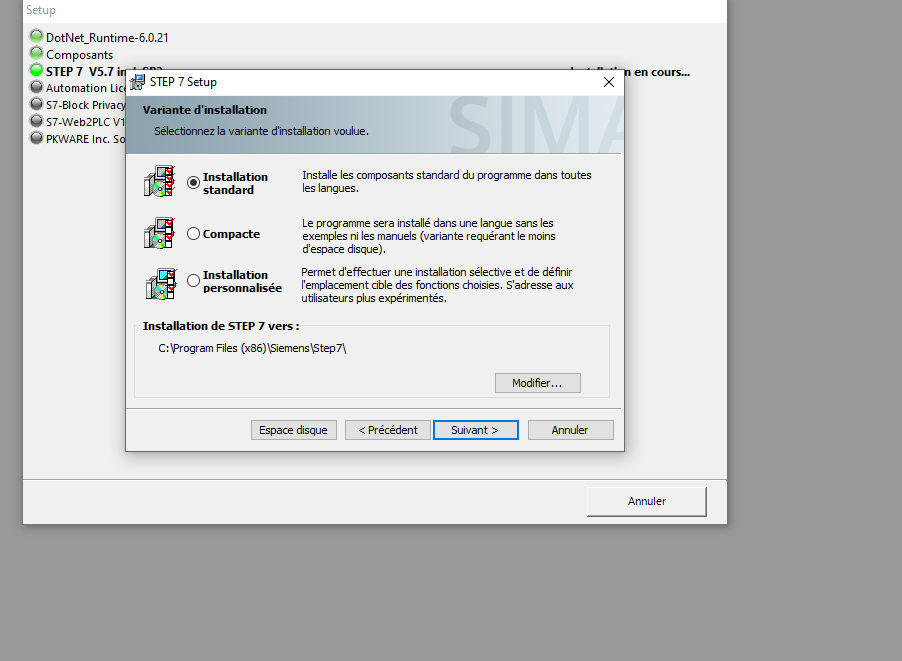
\includegraphics[width=0.72\textwidth]{images/tia-09-step7-v57-installation-standard.png}
    \caption{Assistant d'installation STEP 7 V5.7 incl. SP2 en mode standard.}
\end{figure}

\subsection{Licence STEP 7}

L'assistant de synchronisation des licences a signale que
\texttt{STEP 7-BASIS V5.7} devait disposer d'une licence sur l'ordinateur.
La licence elle-meme ne doit pas etre exportee ni publiee.

\begin{figure}[H]
    \centering
    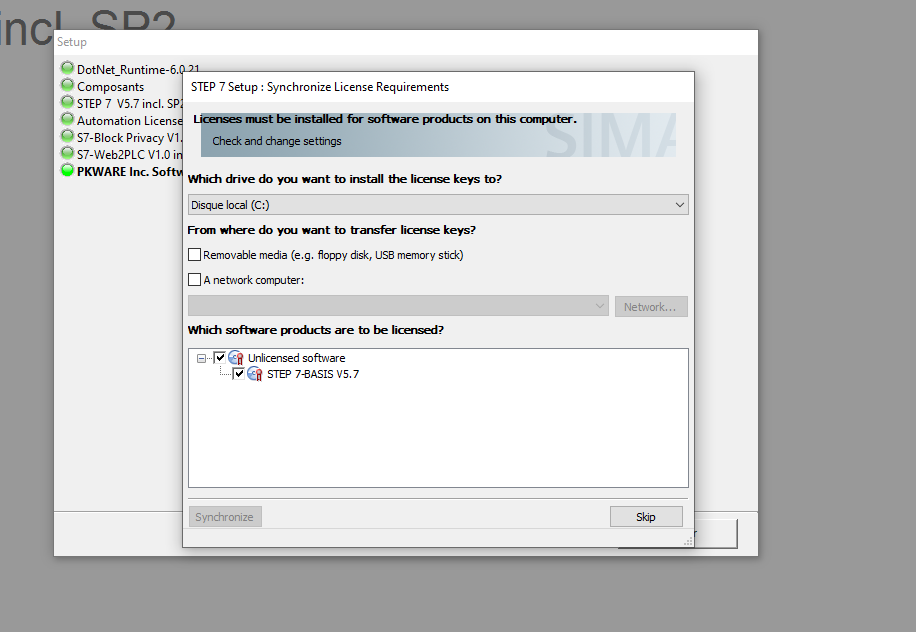
\includegraphics[width=0.72\textwidth]{images/tia-10-step7-v57-licence-a-confirmer.png}
    \caption{Controle de licence STEP 7 V5.7 a confirmer dans Automation License Manager.}
\end{figure}

Le point important est de documenter l'etat sans inclure de cle de licence.
Avant usage prolonge, il faudra verifier dans Automation License Manager
que l'installation correspond bien aux droits disponibles.

% =====================================================
\section{Incidents et diagnostics}
% =====================================================

\subsection{Redemarrage requis par l'installateur}

L'incident principal observe est le redemarrage requis pendant
l'installation TIA Portal. Ce comportement est courant lors d'une
installation lourde Siemens, car plusieurs composants systeme, SQL,
OPC et services Windows sont installes.

Action retenue :

\begin{lstlisting}
Redemarrer la VM Windows.
Relancer les verifications apres ouverture de session.
Verifier les programmes installes dans le Panneau de configuration.
Ouvrir TIA Portal et creer un projet de test.
\end{lstlisting}

\subsection{Licences}

Le document ne contient aucun mot de passe, aucun fichier de licence et
aucune cle. Les captures montrant des ecrans de synchronisation de
licence servent uniquement a documenter le point de controle.

\subsection{Points a verifier avant publication}

\begin{itemize}[leftmargin=*]
    \item confirmer les ressources VMware exactes de la VM ;
    \item confirmer l'etat de licence STEP 7 V5.7 ;
    \item ajouter, si besoin, une capture de \og A propos de TIA Portal \fg{} ;
    \item ajouter, si besoin, une capture des parametres VMware de la VM ;
    \item verifier que les captures ne contiennent aucun chemin personnel ou secret.
\end{itemize}

% =====================================================
\section{Bilan}
% =====================================================

La VM Siemens est utilisable comme poste d'ingenierie du laboratoire.
Windows 10 Pro est installe, TIA Portal V15.1 est lanceable, et les
composants Siemens visibles dans Windows confirment l'installation de
plusieurs briques importantes : Automation License Manager, TIA
Administrator, WinCC Runtime Advanced, TIA Portal Multiuser Server,
ProSave, OPC redistributables et composants SQL.

STEP 7 V5.7 incl. SP2 est documente comme installation lancee avec
controle de licence a confirmer. Les projets Ignition et AVEVA restent
des travaux futurs et ne font pas partie de l'etat installe.

\end{document}
